\documentclass{article}
\usepackage{fullpage}
\usepackage{graphicx} % Required for inserting images
\usepackage{natbib}
\usepackage{hyperref}
\title{Cross-validation with subsets and downsampling for optimizing training in machine learning}
\author{Toby Hocking, 
Daniel Agyapong, Tung Lam Nguyen, David Folch, Bruce Hungate, Jane Marks, Jeffrey Propster, Bilal Aslam, Kevin Gurney, Olivia Lindly
}
\date{February 2026}

\begin{document}

\maketitle


\begin{abstract}
In machine learning, training data sometimes comprise natural subsets defined by categorical variables such as geographic region, time period, or demographic group. 
SOAK framework of Hocking et al.\ (2026) addresses the question of which training subset yields the best model, but leaves open a subtler problem: when subsets differ in size, it is unclear whether performance gaps are driven by the origin of the data or by the amount of it.
We propose SOAKED (Same/Other/All K-fold cross-validation Extension: Downsampling), which extends the SOAK framework by incorporating random downsampling to equalize training set sizes across the same, other, and all configurations. 
With this approach, one can differentiate two distinct drivers of performance: one stemming from real distributional differences between subsets, and another that simply reflects the fact that some subsets have more training data than others.
We demonstrate SOAKED on simulated regression data, benchmark classification tasks (STL10, waveform), survey data (NSCH autism), qSIP biological data, carbon emissions data, and income data. 
Our results show that in some data sets, downsampling eliminates performance differences, confirming a sample size effect, while in others, differences persist, revealing a true subset effect. 
An implementation is available in the \texttt{mlr3resampling} R package, enabling users to go beyond SOAK by incorporating downsampling to cleanly separate the effect of subset choice from the effect of training set size.
\end{abstract}


\section{Introduction}
In many real-world applications of machine learning, we work with datasets that naturally fall into distinct subsets defined by categorical variables such as temporal period, geographic region, or data collection protocol. 
A fundamental question arises in such settings that when we observe differences in model performance across these subsets, can we determine whether these differences come from genuine distributional divergence between subsets, or whether they simply reflect the fact that some subsets contain more training data than others?

For example, consider a public health surveillance system that develops models using data from two consecutive years of data collection. 
Should we train using only the current year (same subset), using data from previous years (other subsets), or using all available data (all subsets)? 
If the model trained on all years performs better, is this improvement due to combining complementary patterns from different years, or merely because we have more training examples? 
This distinction matters practically because if the gain comes solely from data volume, then prioritizing data collection from underrepresented years would be beneficial. 
Conversely, if real distributional shifts exist between years, we might need distributional robustness techniques.

The SOAK framework \citep{hocking2026} addresses part of this challenge by systematically comparing models trained on same, other, and all subset configurations. However, SOAK leaves an important technical problem unresolved about subsets that differ substantially in size, the framework does not cleanly separate subset effects (distributional differences) from sample size effects (performance gains due to more training data).

We propose SOAKED (\textbf{S}ame/\textbf{O}ther/\textbf{A}ll \textbf{K}-fold cross-validation \textbf{E}xtension: \textbf{D}ownsampling), which extends SOAK by incorporating random downsampling to equalize training set sizes across same, other, and all configurations. 
By holding training set cardinality constant across these three scenarios, SOAKED decouples two distinct mechanisms driving model performance: (1) the subset effect, reflecting genuine differences in learnable patterns between subsets, and (2) the sample size effect, reflecting the well-documented phenomenon that model performance improves as training set size increases. 
By isolating the subset effect from the sample size effect, we can confidently identify fundamental data heterogeneity rather than artifacts of imbalanced data collection.

We demonstrate SOAKED across a diverse collection of datasets: simulated regression problems with known distributional structure, benchmark classification datasets (STL10, waveform), epidemiological survey data (NSCH autism), microbial biogeochemistry data (qSIP), climate data (carbon emissions), and economic data (income prediction). Our empirical findings reveal substantial heterogeneity: in some datasets, downsampling eliminates observed performance gaps, confirming that subset-size imbalance was the primary driver; in others, performance differences persist despite equal training set sizes, indicating genuine subset effects that warrant special modeling attention.




\section{Related work}

\subsection{Internal and External validation}
% To summarize, internal holdout data would come from a sequestered portion of the original dataset, while the external validation data would come from a different data source/population.
 
% Internal Validation
	
% Evaluation of model or analytic performance within the original dataset using resampling or partitioning methods (e.g., cross-validation, bootstrapping)18,19.
	
% A model is internally validated if its performance remains stable using samples within the development dataset.

% External Validation 
	
% Testing a model on a sample taken from a population different than the original cohort to determine whether the model works to a satisfactory degree18,19.
	
% A model is externally validated if it is consistent in a similar study conducted using samples from a different population.


% We are definitely at least doing internal validation.

% I’m not sure if we are doing external validation. It depends on the definition of "different data source/population."
% We have two different years of data from National Survey of Children’s Health.
% Those are two different data files, with two different groups of people surveyed.
% (but both groups of people are supposed to be representative of the overall USA population)
% Is that an example of External Validation? or not?


\subsection{Spatio-temporal cross-validation}

The mlr3spatiotempcv R package provides an interface to a variety of different cross-validation methods, all of which require data spatial coordinates \citep{schratz2024}.
It discusses an example involving crop classification from satellite data, with 100 fields (each containing 20 grid cells) spread over several geographical regions.
It is desirable to hold out data at the level of fields, not grid cells (so field would be assigned column role group in mlr3).
SOAK can be used in this context, by assigning subset role to a categorical column representing a geographical region ID, and by assigning group role to a column with the field ID.
In this context, \citet{brenning2005} refers to SOAK subsets as ``domains,'' so the SOAK Other model is ``extra-domain prediction'' whereas the Same model is ``intra-domain prediction.''
In mlr3spatiotempcv the term ``block'' is used for a contiguous spatial area, typically used as column role group (data in a group/block are not split in CV).
The blockCV R package provides several algorithms (blocking, clustering, etc.) for creating fold IDs based on spatial coordinates \citep{valavi2019}, when the data do not already have pre-defined group/block IDs like field in the satellite data example.

\begin{tabular}{cccc}
problem & rows & group & subset \\
\hline
crop classification & grid cells & fields & region \\
tree classification & pixels & polygons & region
\end{tabular}

\section{Data sets}
\subsection{Carbon emissions}
These data combine Average Annual Daily Traffic (AADT) from the USA Highway Performance Monitoring System (HPMS) \citet{bilal_hpms_aadt}, WorldPop population \citet{bilal_worldpop}, OpenStreetMap road density \citet{bilal_osm_roads}, Sentinel-2 imagery \citet{bilal_sentinel2}, and VIIRS night-time lights \citet{bilal_ntl_viirs}.


\section{Methods}


\begin{figure}
    \centering
    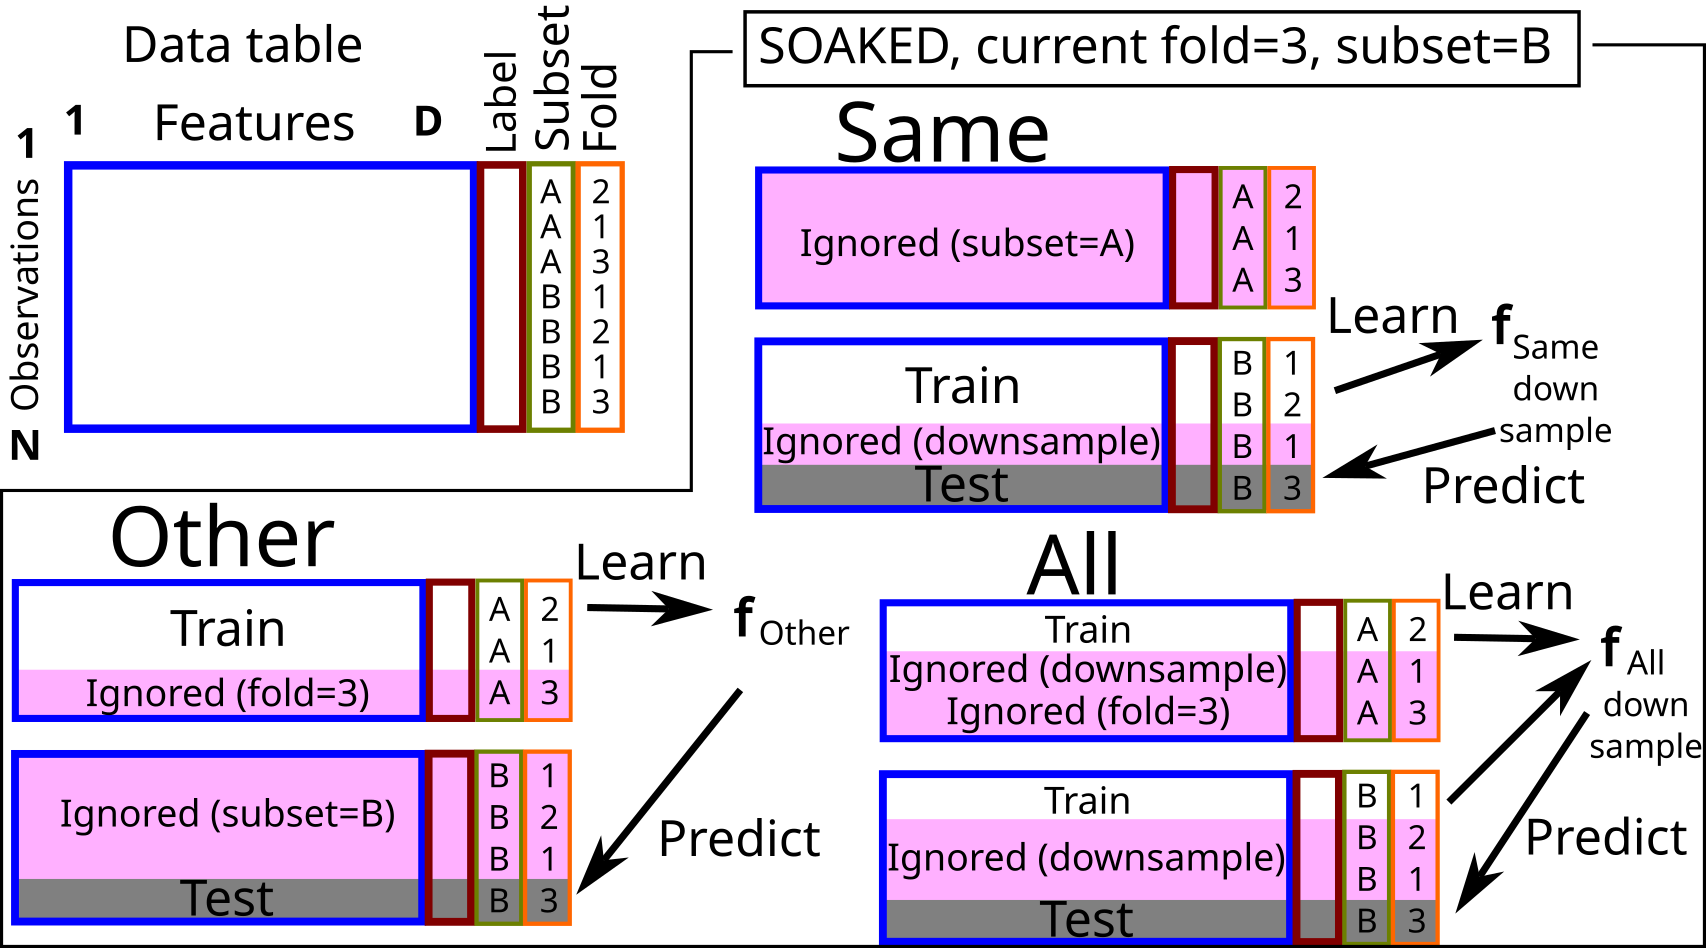
\includegraphics[width=0.8\linewidth]{drawing-SOAKED-generic.png}
    % https://github.com/tdhock/cv-same-other-paper/blob/main/slides/drawing-SOAKED-generic.svg
    \vskip -1cm
    \caption{
    SOAKED algorithm for test fold=3 and test subset=B in data with two subsets of different sizes: A has three rows and B has four rows.
    After excluding data based on fold and subset, random downsampling is used for Same and All models, to obtain train sets of size equal to the smallest train set (Other, 2 rows).
    }
    \label{fig:SOAKED-concept}
\end{figure}

\paragraph{Sample size effect.}
When the subset(s) used for training (either \textit{same}, \textit{other} or \textit{all}) is fixed, model performance improves as the number of training samples increases. 
In other words, models trained on more training samples consistently perform better. 
This indicates that regression models benefit from increased data availability, likely because additional samples allow the model to better capture the underlying data distribution and reduce variance.

\paragraph{Subset effect.}
When the training sample size is fixed, the model trained on the \textit{same} subset performs best, followed by the model trained on the \textit{all} subsets, and finally the model trained on the \textit{other} subset. 
This suggests that there are differences in the underlying patterns between the two gender subsets, making models trained on the \textit{same} subset better.
However, when using the full size dataset, the model trained on the \textit{all} subsets performs slightly better than the full-size \textit{same} model. 
This indicates that although the subsets have distinct patterns, they are still partially related. 
As a result, incorporating additional samples from the \textit{other} subset can still contribute useful information and lead to a small improvement in overall model performance.
\section{Results}

\subsection{Simulated regression data sets}
TODO Toby explain setup and results.

\begin{figure}
    \centering
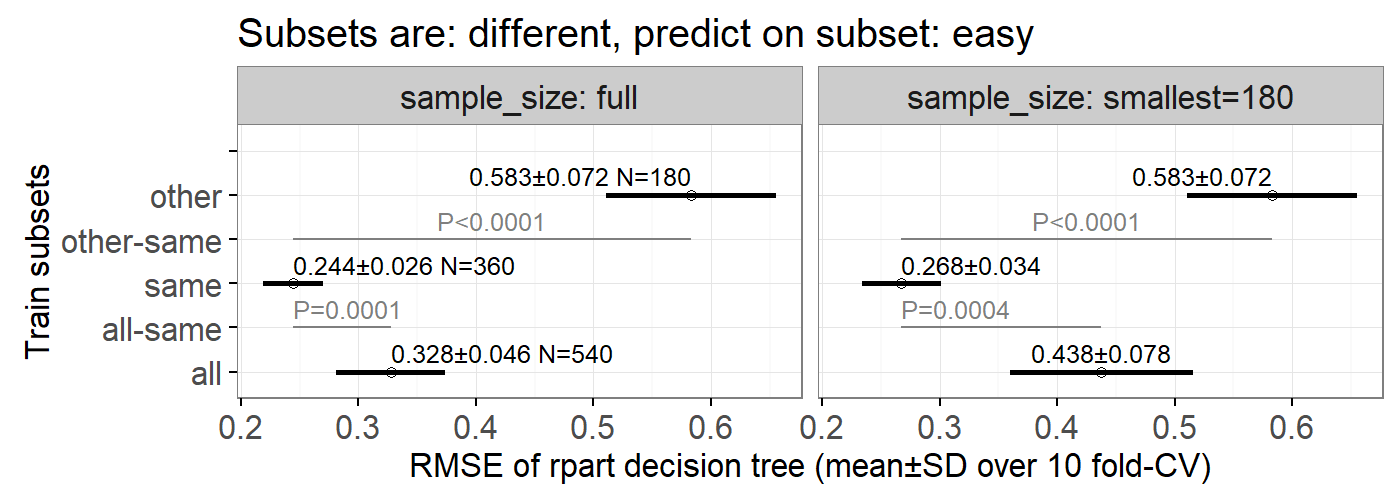
\includegraphics[width=0.8\textwidth]{cv-subsets-small-large-noise-different-easy.png}
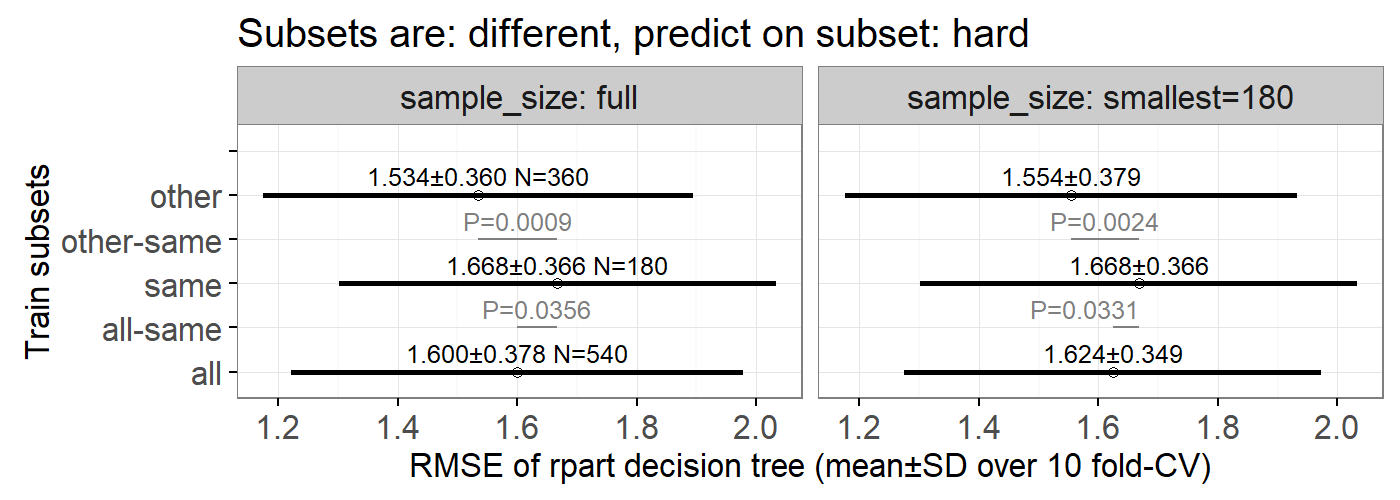
\includegraphics[width=0.8\textwidth]{cv-subsets-small-large-noise-different-hard.png}
% https://github.com/tdhock/2024-08-ift603-712/blob/main/cv-subsets-small-large-noise.R
    \caption{Results of using SOAKED on simulated data with two subsets with a different (but consistent) pattern, and with different numbers of samples.}
    \label{fig:sim-different}
\end{figure}

\begin{figure}
    \centering
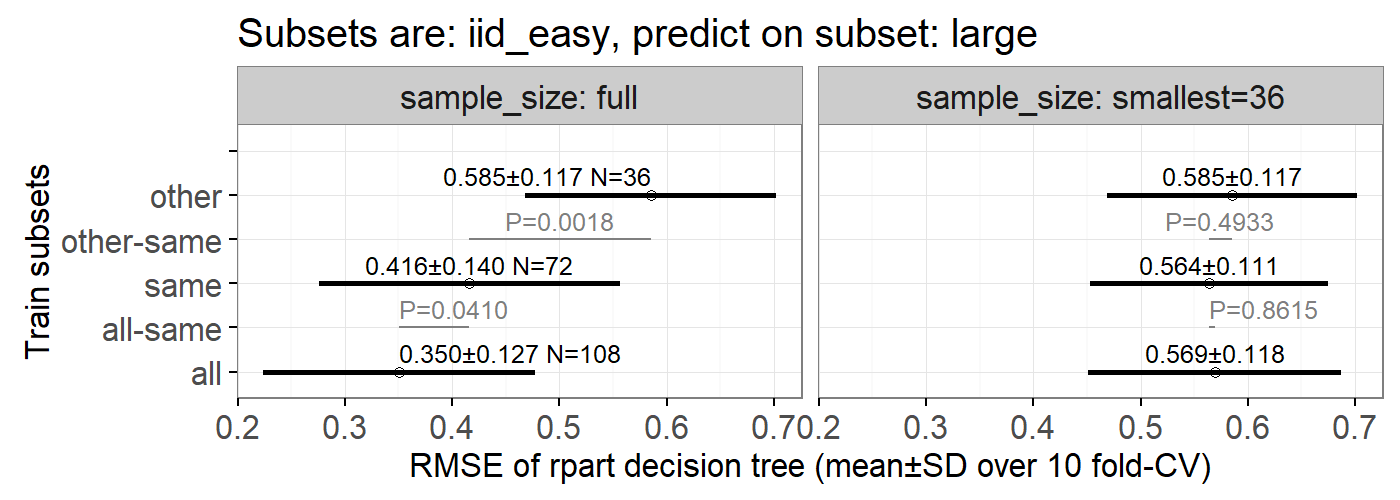
\includegraphics[width=0.8\textwidth]{cv-subsets-small-large-noise-iid_easy-large.png}
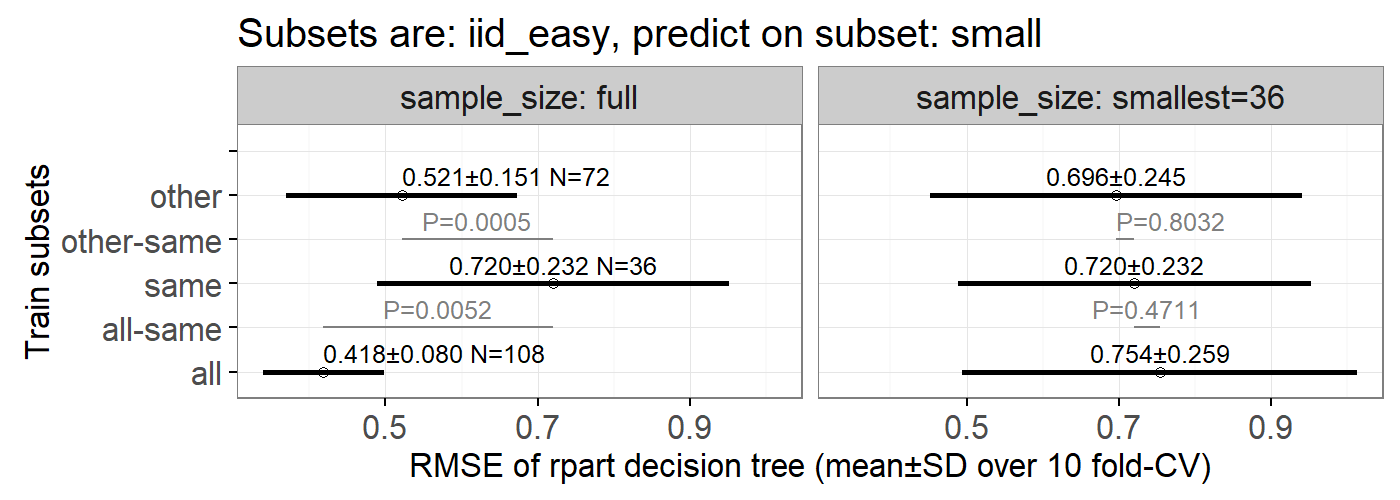
\includegraphics[width=0.8\textwidth]{cv-subsets-small-large-noise-iid_easy-small.png}
% https://github.com/tdhock/2024-08-ift603-712/blob/main/cv-subsets-small-large-noise.R
    \caption{Results of using SOAKED on simulated data with two subsets that are i.i.d. but with different numbers of samples.}
    \label{fig:sim-iid}
\end{figure}

\subsection{Benchmark classification data sets}
TODO Toby explain examples from SOAK paper.


\begin{figure}
    \centering
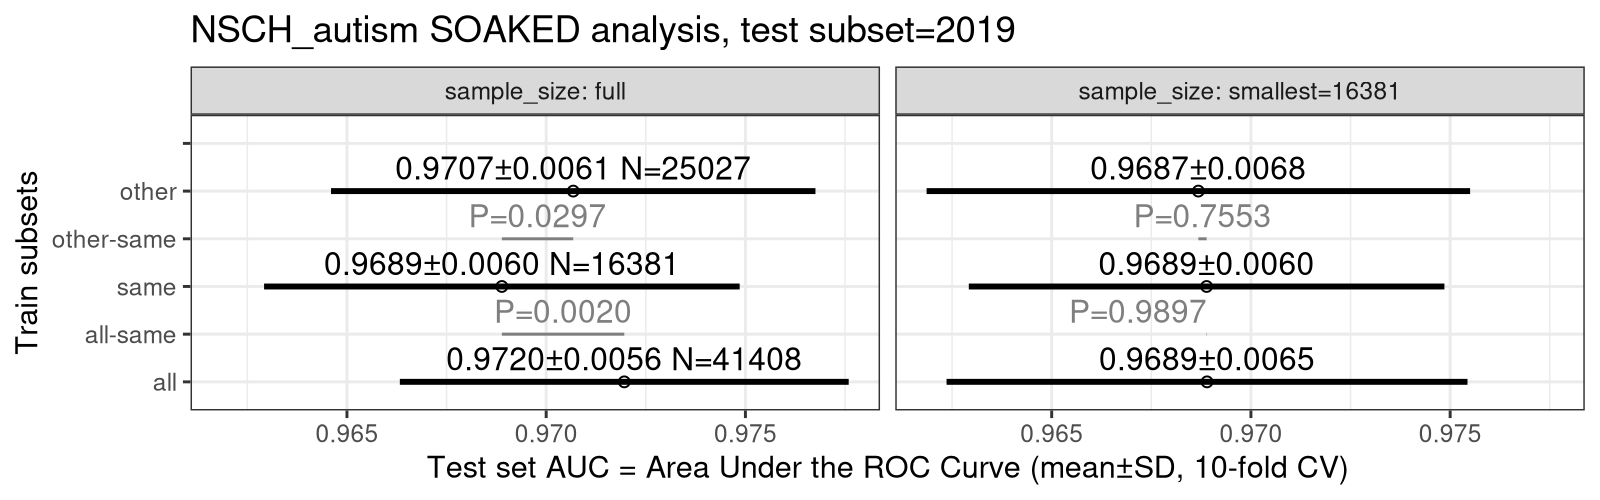
\includegraphics[width=0.8\textwidth]{NSCH_autism_reproduce_downsample_2019.png}
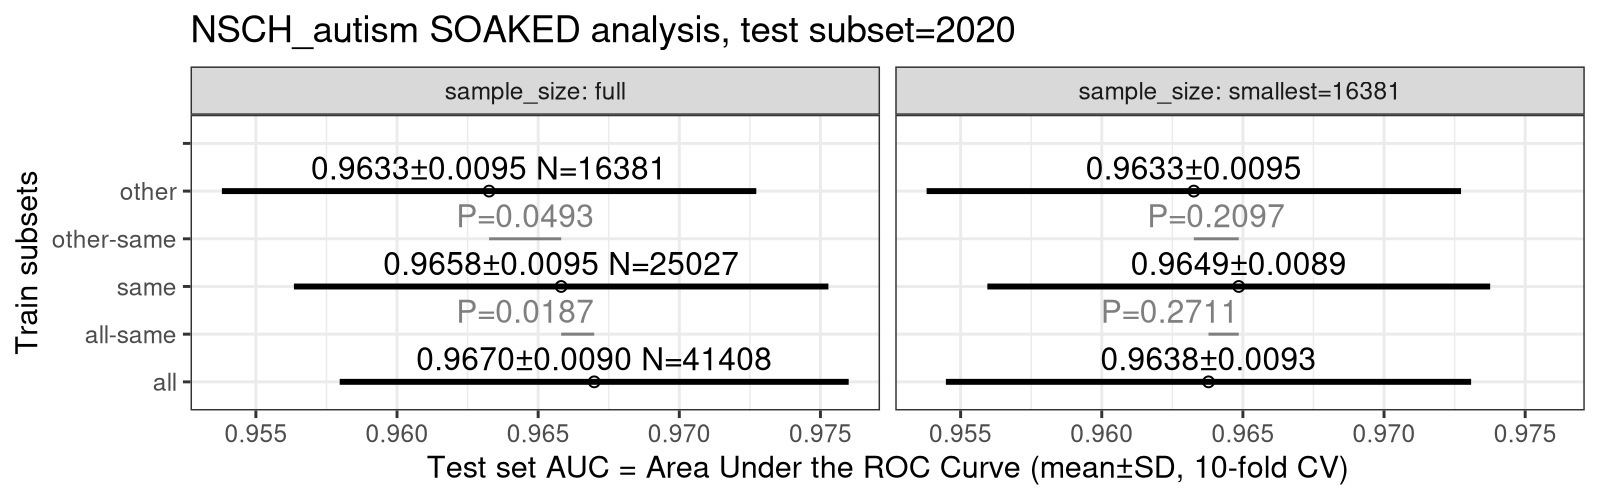
\includegraphics[width=0.8\textwidth]{NSCH_autism_reproduce_downsample_2020.png}
% https://github.com/tdhock/cv-same-other-paper/blob/main/NSCH_autism_reproduce_downsample.R
\caption{Results of using SOAKED on NSCH\_autism data with two subsets (years), each with a different number of samples.}
   \label{fig:NSCH_autism}
\end{figure}

\begin{figure}
    \centering
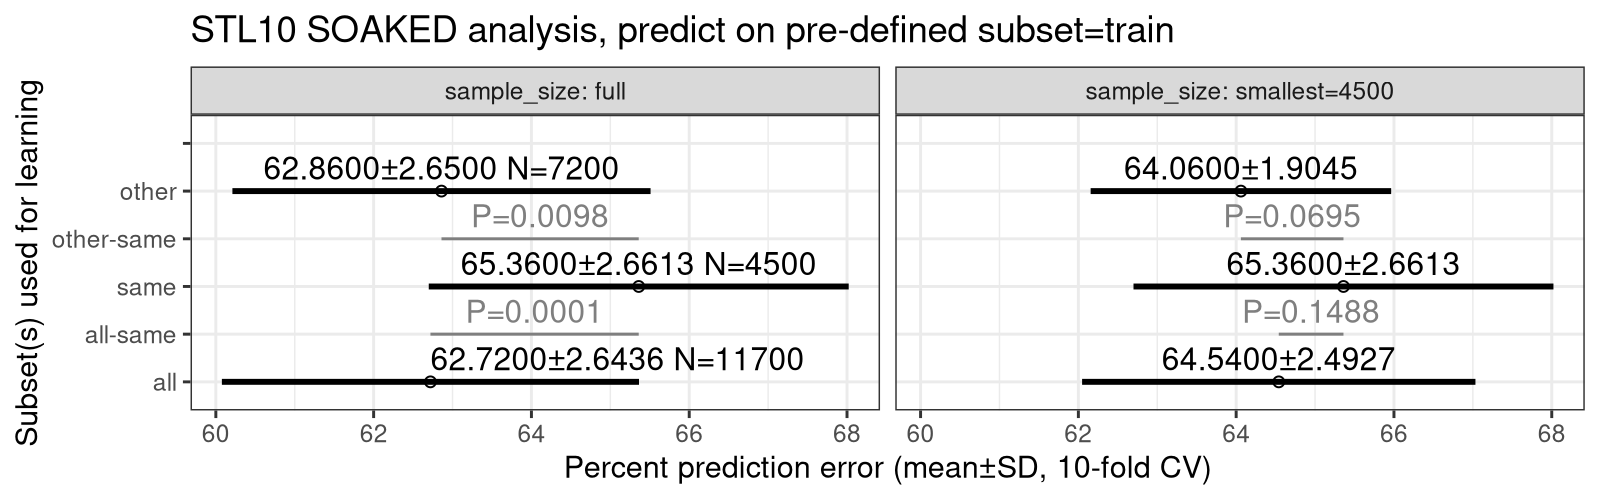
\includegraphics[width=0.8\textwidth]{SOAKED_STL10_waveform_figure_STL10_train.png}
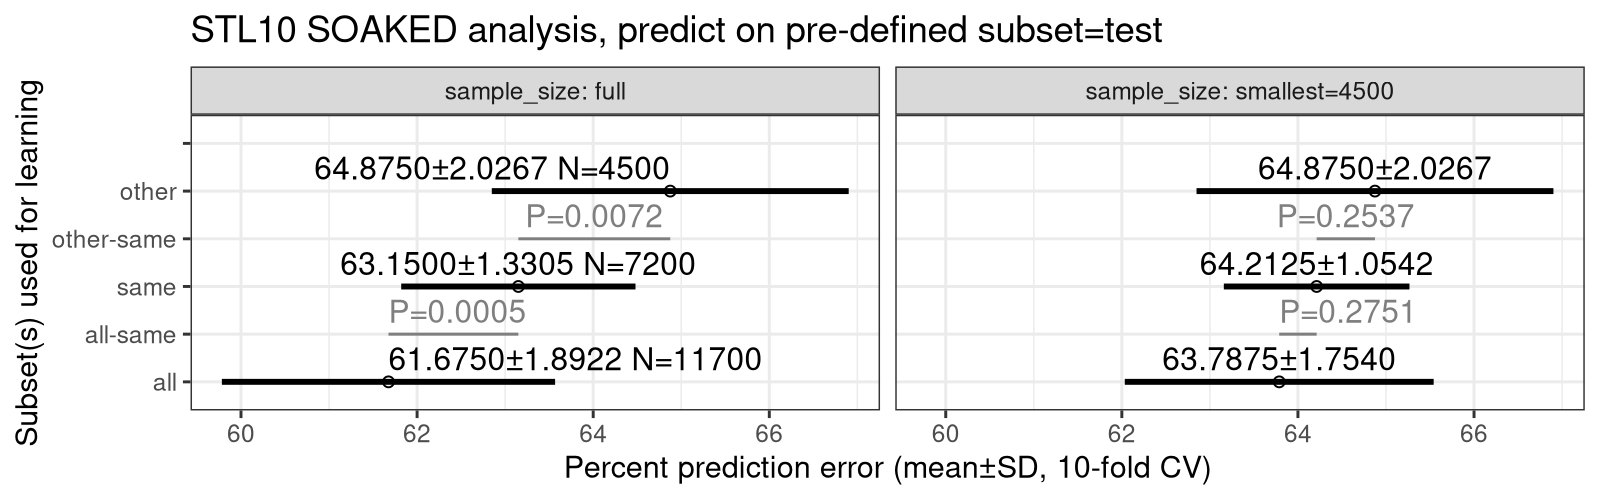
\includegraphics[width=0.8\textwidth]{SOAKED_STL10_waveform_figure_STL10_test.png}
% https://github.com/tdhock/cv-same-other-paper/blob/main/SOAKED_STL10_waveform_figure.R
\caption{Results of using SOAKED on STL10 data with two subsets (pre-defined train/test split), each with a different number of samples.}
   \label{fig:STL10}
\end{figure}

\begin{figure}
    \centering
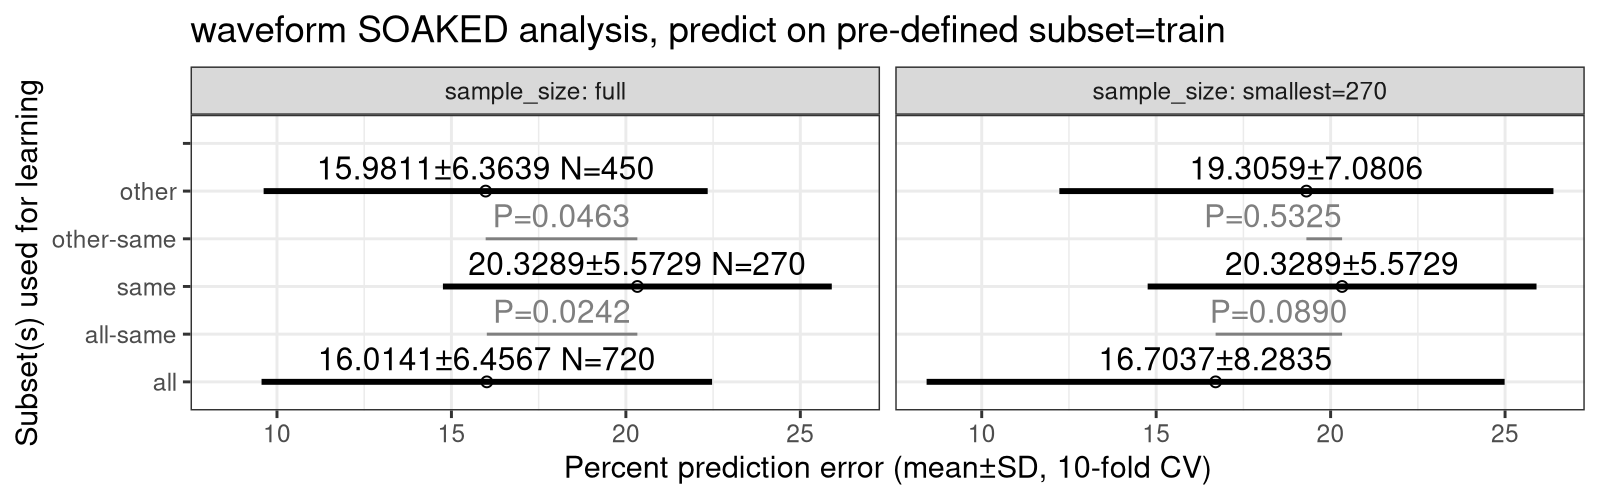
\includegraphics[width=0.8\textwidth]{SOAKED_STL10_waveform_figure_waveform_train.png}
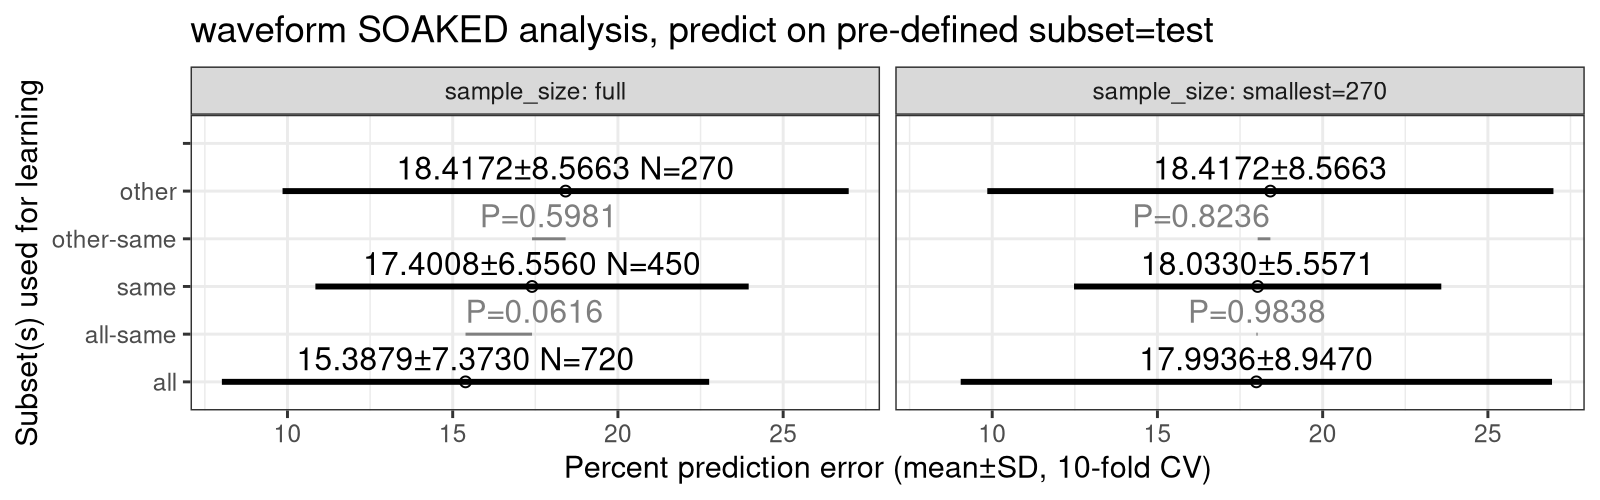
\includegraphics[width=0.8\textwidth]{SOAKED_STL10_waveform_figure_waveform_test.png}
% https://github.com/tdhock/cv-same-other-paper/blob/main/SOAKED_STL10_waveform_figure.R
\caption{Results of using SOAKED on waveform data with two subsets (pre-defined train/test split), each with a different number of samples.}
   \label{fig:waveform}
\end{figure}


\subsection{qSIP regression data sets}
TODO Dan and Jeff explain context and results.

\subsection{Carbon emissions regression data sets}
TODO Bilal explain context.

\subsection{Regression data sets with gender subsets}
% https://raw.githubusercontent.com/lamtung16/soak_regression/refs/heads/main/results/WorkersCompensation/Gender.csv
The Workers Compensation dataset \cite{Ali2020} is a tabular dataset consisting of 100,000 synthetically generated insurance claims. 
Each record represents a realistic worker compensation claim described by 14 features, including the initial case estimate, accident and reporting dates, demographic information of the worker, and a brief text description of the accident. 
The primary prediction target is the UltimateIncurredClaimCost, representing the final financial loss of the claim. 
For the purposes of evaluating model performance across demographic groups (SOAK split), the Gender attribute is utilized. 
The dataset exhibits a notable imbalance within this subset, containing 77,020 male instances and 22,980 female instances. 
This data was provided by Colin Priest (\href{https://github.com/colinpriest}{GitHub}) and, while related, is not the same as the one on \href{https://www.kaggle.com/c/actuarial-loss-estimation}{Kaggle}.

\subsection{Summary of results across all data sets}
\begin{table}[]
    \centering
    \begin{tabular}{c|c|c|c|c|c|c}
data  & test subset & accuracy & train sizes & Scenario & acc. w/ downsample & conclusion \\
\hline
iid\_easy & small & $s<o<a$ & $s<o<a$ & Om & $s=o=a$ & sample size \\
iid\_easy & large & $o<s<a$ & $o<s<a$ & Sm & $s=o=a$ & sample size  \\
different & hard & $s<a<o$ & $s<o<a$ & Oi & $s<a<o$ & subset \\
different & easy & $o<a<s$ & $o<s<a$ & Si & $o<a<s$ & subset  \\ 
NSCH\_autism & 2019 & $s<o<a$ & $s<o<a$ & Om & $s=o=a$ & sample size \\
STL10 & test & $o<s<a$ & $o<s<a$ & Sm & $s=o=a$ & sample size  \\
waveform & test & $o<s<a$ & $o<s<a$ & Sm & $s=o=a$ & sample size  \\
qSIP & qme.15 & $o<a<s$ & $o<s<a$ & Si & $o<a<s$ & subset \\
income & M & $o<a=s$ & $o<s<a$ & S & $o<a=s$ & subset
\end{tabular}
    \caption{Scenario codes: O: $s<o$ for accuracy and train size,
S: $o<s$ for accuracy and train size,
m: all has max accuracy,
i: all has intermediate accuracy.
}
    \label{tab:placeholder}
\end{table}


\bibliographystyle{abbrvnat}
\bibliography{refs}
\end{document}
